\chapter{Coordination ATL}
Une entrée dédicacée à la coordination ATL a été ajoutée sur le portail. Via cette entrée, toutes les informations utiles à la fonction de CATL et à la subvention des CATL sont disponibles. 

\section{Entrée - Ma Commune}
Développez le volet de coordination ATL (volet de navigation à gauche) et cliquez sur l’entrée « Ma Commune ». Cette entrée se décline en 2 onglets: Tableau de bord et Contact ONE.



\subsection{Onglet - Tableau de bord}
Le tableau de bord du premier onglet vous permet d’avoir une vue sur : 

\begin{itemize}
\item Les différentes activités ATL agrées/reconnues (màj en temps réel);
\item Les informations relatives à la démographie de votre commune (màj annuelle);
\item Le nombre d’implantations scolaires par réseau d’enseignement (màj régulièrement). 
\end{itemize}

%ajouter le logo
En cliquant sur 
\includegraphics[width=0.4cm]{Images/icon/consult_ma_commune.png}, vous aurez le détail de chaque secteur. 

\begin{conseil}
 Si vous constatez une erreur à ce niveau, n’hésitez pas à entrer en contact avec votre référente agrément ou le support administratif de la cellule agrément. 
\end{conseil}


\begin{figure}[htbp]
    \centering
    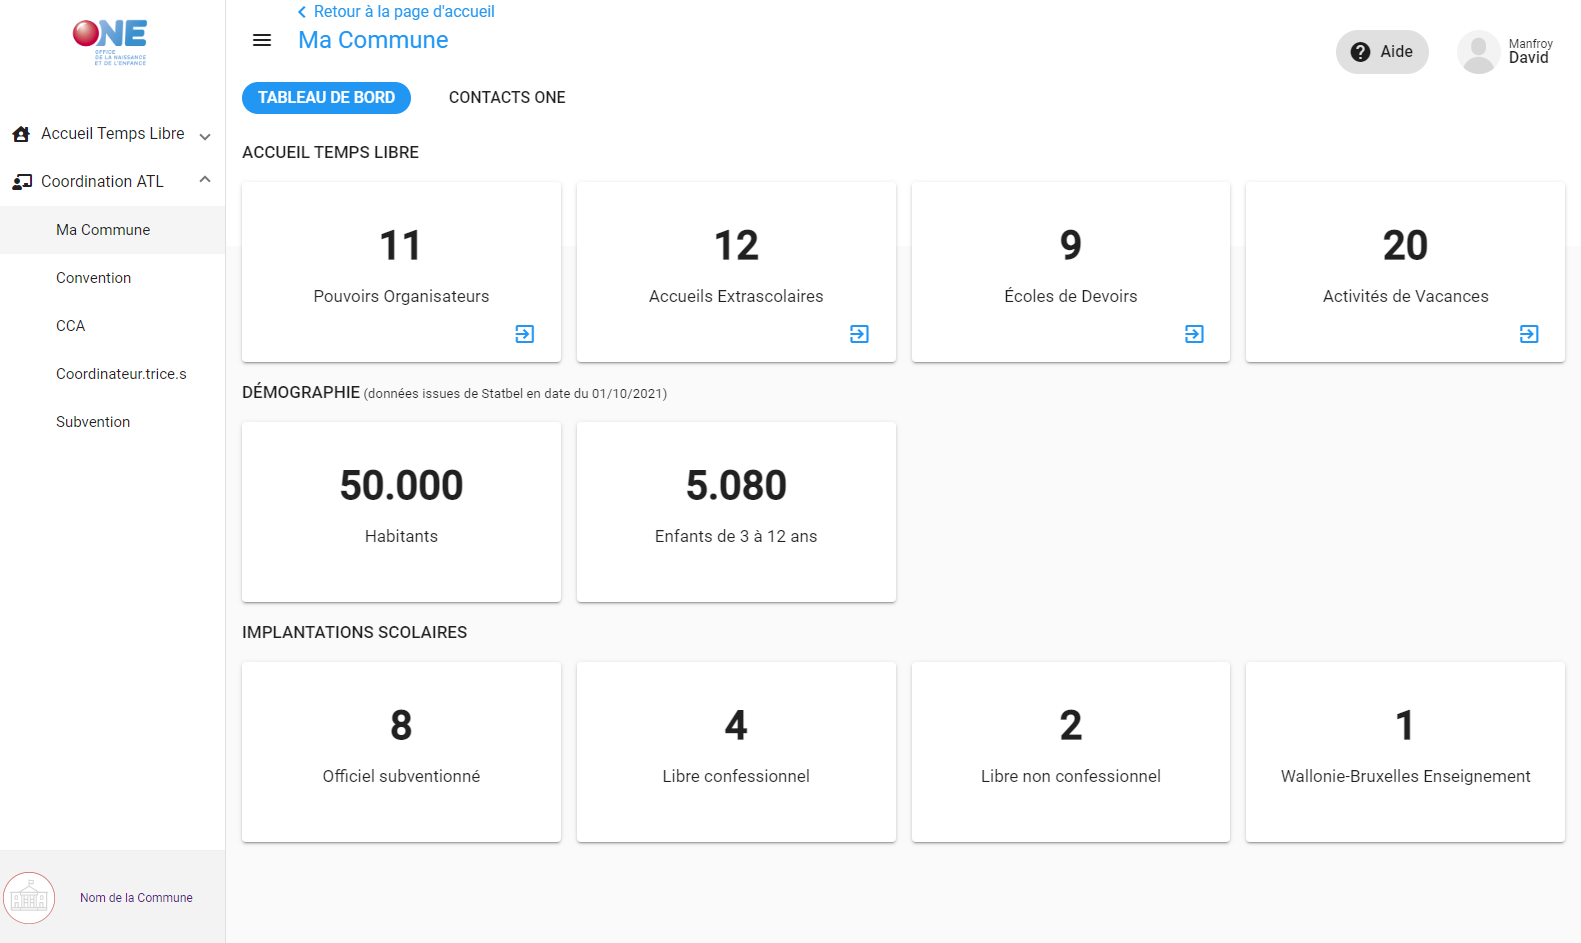
\includegraphics[width=12cm]{Images/catl/Ma Commune.png}
    \caption{Le tableau de bord de 'Ma Commune' présente des informations comme le nombre d'activités et lieux ATL sur le territoire communal, des données statistiques, etc.}. Il ne renseigne pas les accueil qui ont remplit une déclaration d'accueil auprès de l'ONE.
    \label{fig:ma_commune}
\end{figure}




\subsection{Onglet - Contacts ONE}
Le second onglet « Contacts ONE », vous permet de retrouver les coordonnées des agents de l’ONE attitrés à la coordination ATL de votre commune. 



\section{Entrée - Convention}
Dans ce volet, vous trouverez tout ce qui concerne la convention. Cette entrée se décline également en 3 onglets: convention, demande de modification et ressources.



\subsection{Onglet - Convention}
Dans cet onglet, vous retrouverez tout ce qui touche à la convention ATL signée entre votre commune et l’ONE.

\subsubsection{Documents reçus de l'ONE}
 Sur cette page, vous trouverez un encart composé de toutes les conventions et les éventuels avenants signés ainsi que les courriers de notification qui s’y rattachent. Vous pourrez télécharger les pièces et consulter certaines informations (temps de travail subventionné, missions spécifiques, délégation de coordination)

\begin{figure}[htbp]
    \centering
    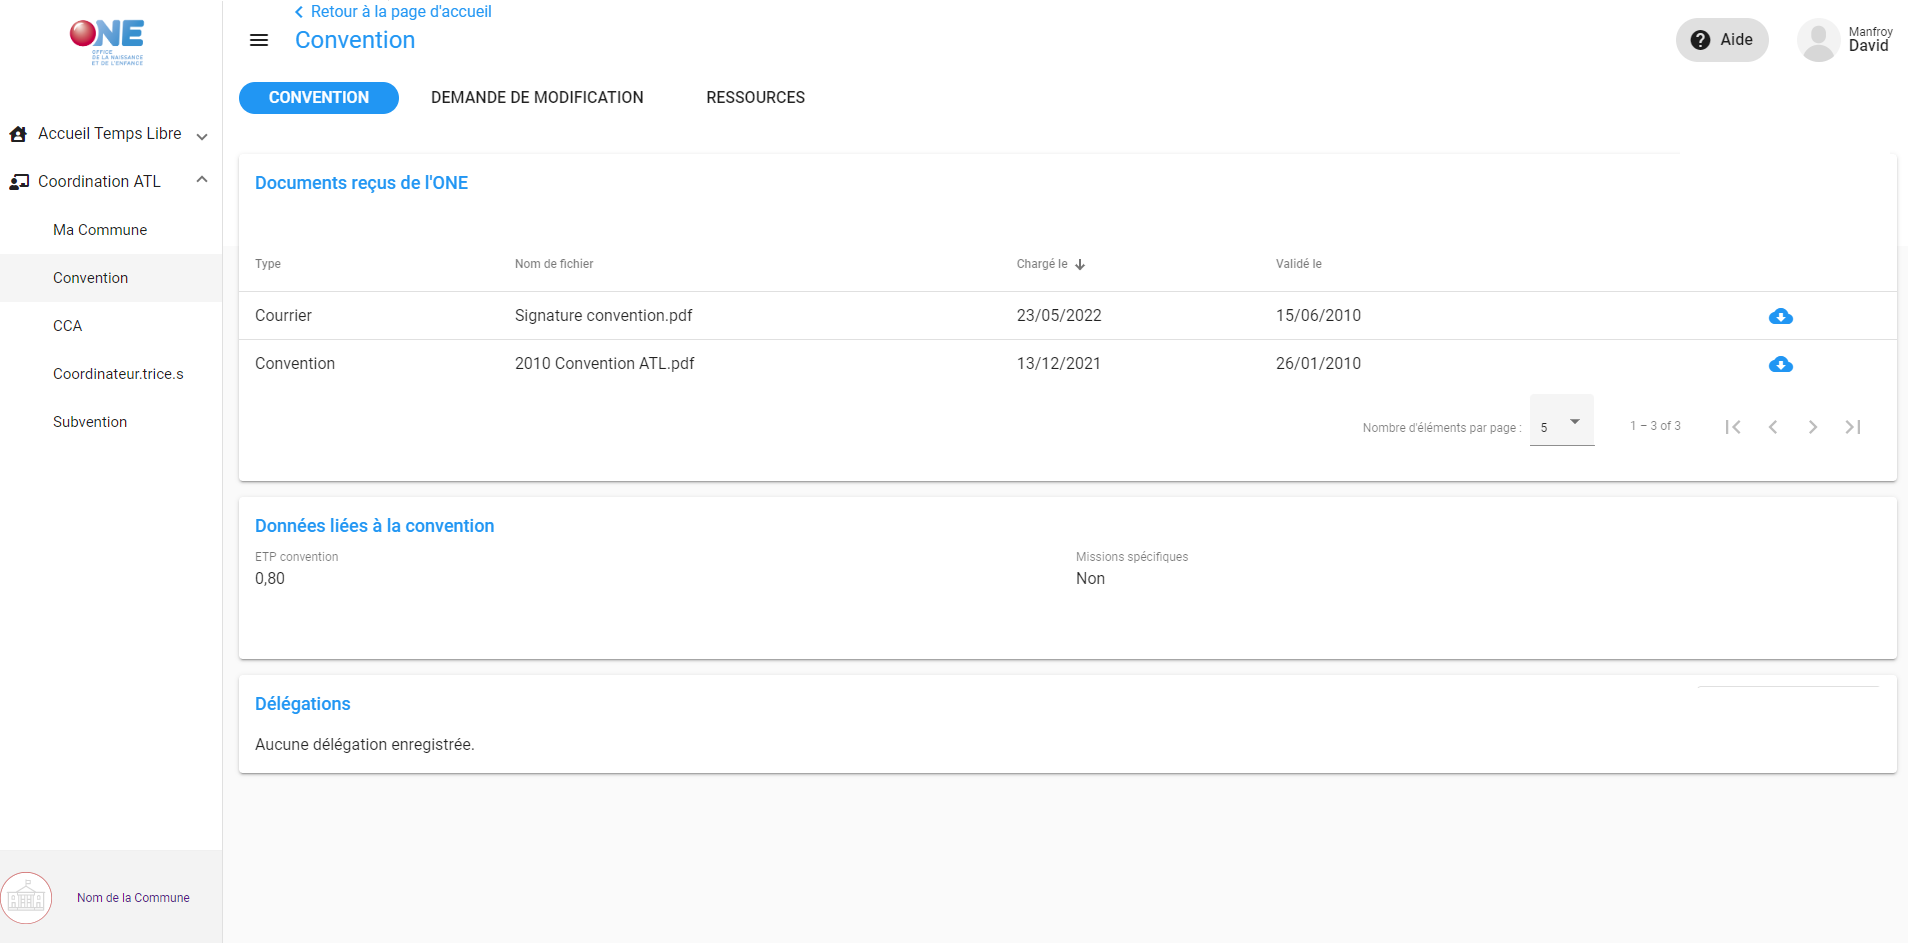
\includegraphics[width=11cm]{Images/catl/Convention.png}
    \caption{L'entrée Convention donne une vue d'ensemble de la convention ATL-ONE.}
    \label{fig:convention_catl}
\end{figure}


\subsubsection{Données liées à la convention}
Cet encart précise le temps de travail subventionné et mentionné dans la convention et si des missions spécifiques vous sont attribuées ou non sur ce même temps de travail (fig. \ref{fig:convention_etp_mission}). 

\begin{figure}[h!]
    \centering
    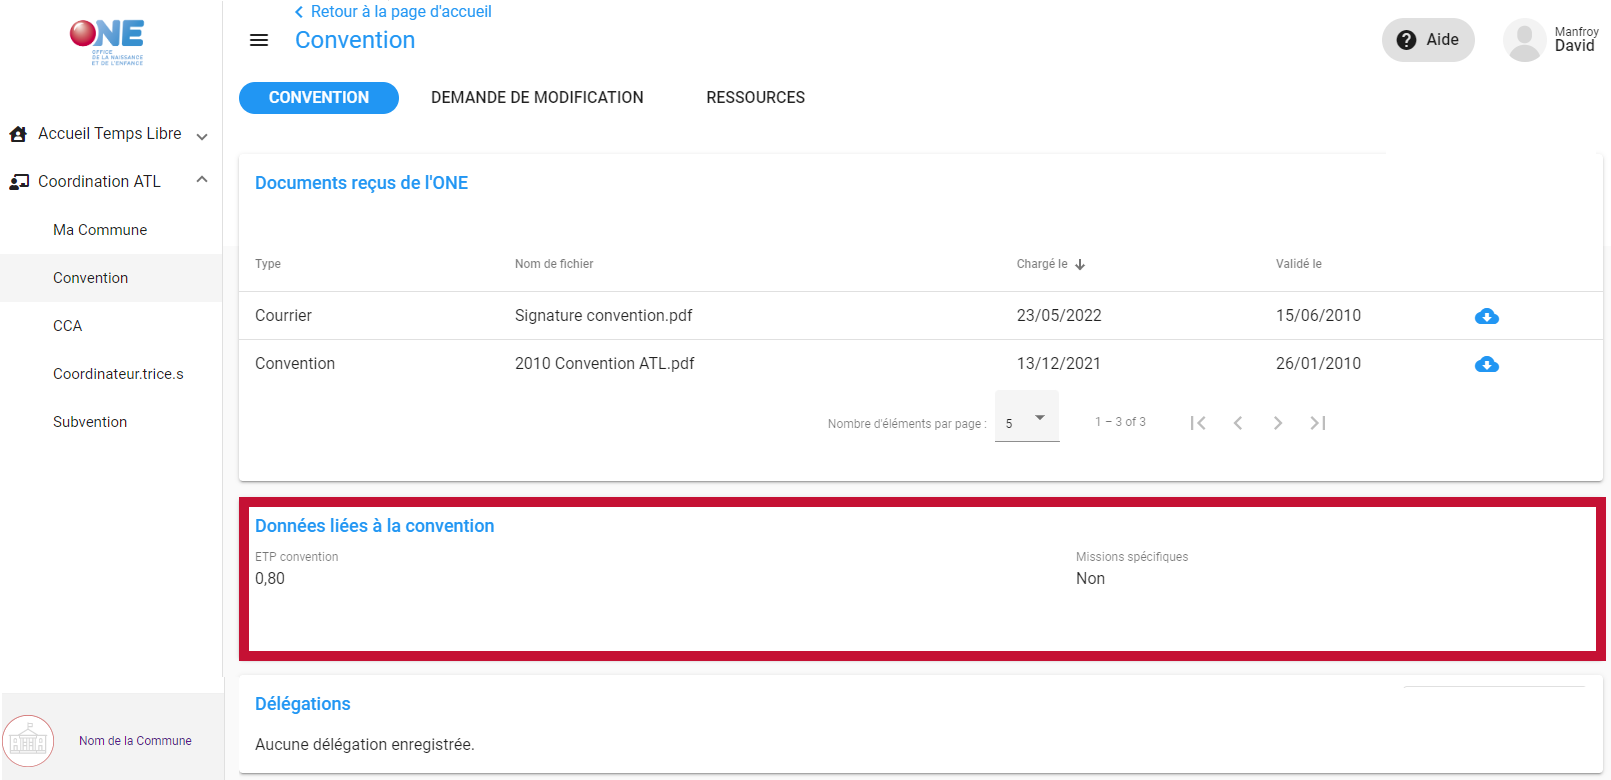
\includegraphics[width=9cm]{Images/catl/Convention-etp-missions.png}
    \caption{Le cadre }
    \label{fig:convention_etp_mission}
\end{figure}

\subsubsection{Délégation de coordination ATL (ASBL)}
Lorsqu’une commune décide de déléguer la coordination ATL à une ASBL, c’est également ici que vous retrouverez l’identité de l’ASBL de délégation. 

\subsection{Onglet - Demande de modification de la convention}
Que cela soit au moyen d’un avenant ou d’une actualisation complète de la convention, vous devrez à présent introduire votre demande via le portail. Pour se faire, cliquez sur « Demande de modification » et chargez les documents obligatoires, à savoir : 

\begin{itemize}
    \item La demande de modification de convention signée par les autorités communales 
    \item L’extrait aux registres des délibérations du conseil communal approuvant ledit document 
\end{itemize}

Une zone de chargement est disponible pour l’envoi de ces documents. 

\begin{figure}[htbp]
    \centering
    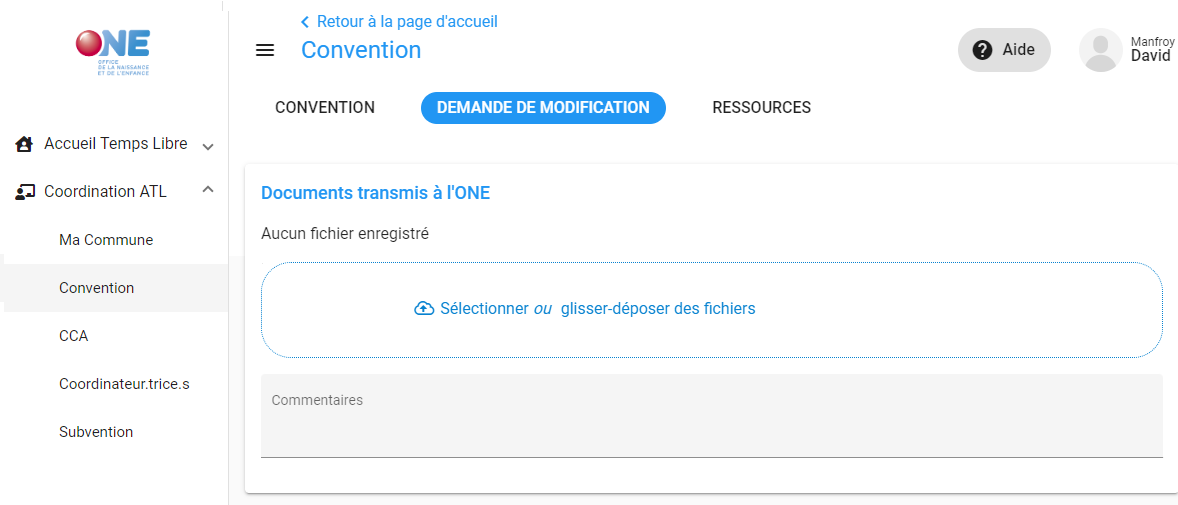
\includegraphics[width=12cm]{Images/catl/Demande de modification.png}
    \caption{L'onglet demande de modification permet de transmettre à l'ONE les documents relatifs aux amendements de la convention.}
    \label{fig:dmd_modif_convention}
\end{figure}


\begin{attention}
Pour l’instant, l’ONE n’est pas informé de ces chargements, il convient donc d’envoyer un mail au support administratif afin de prévenir de l’introduction d’une demande de modification de la convention.
\end{attention}

\subsection{Onglet - Ressources}
Cet onglet vous permettra de télécharger : 
\begin{itemize}
    \item Une \textbf{version Word de la convention complète} : cette version contient des commentaires qui vous guideront dans vos démarches
    \item Une \textbf{version Word d’un avenant à la convention}: cette version contient également des commentaires qui vous guideront dans cette démarche
    \item Une \textbf{description de fonction du CATL} qui est une annexe faisant partie intégrante de la convention 
\end{itemize}



\begin{figure}
    \centering
    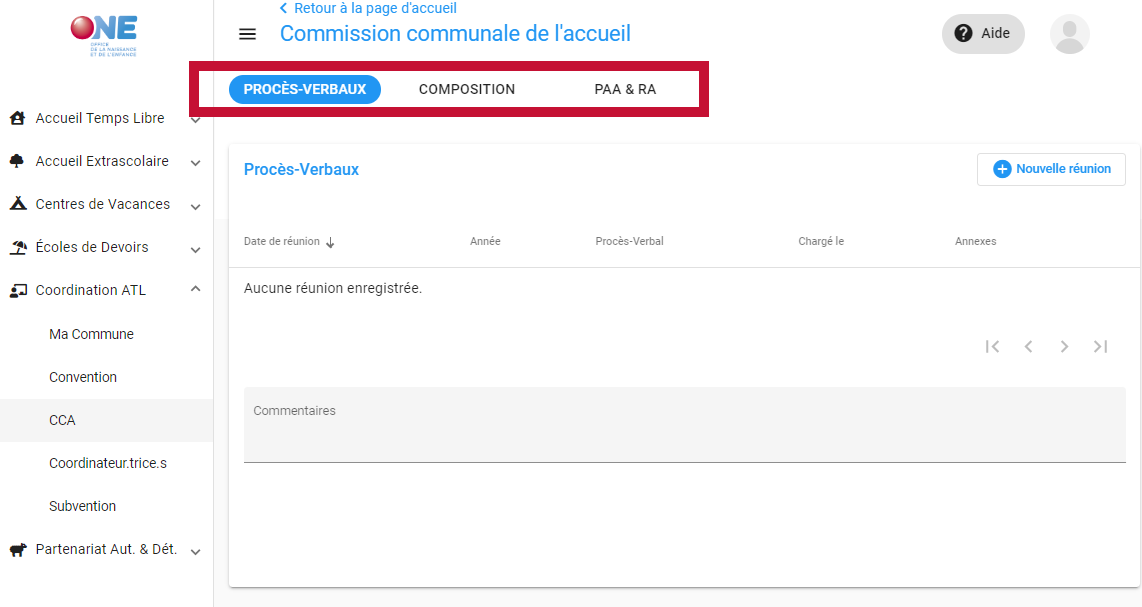
\includegraphics[width=0.5\linewidth,frame]{Images/catl/cca-onglets.png}
    \caption{L'entrée CCA avec les 3 onglets}
    \label{fig:cca-onglets}
\end{figure}

\section{Entrée - CCA - Commission Communale de l'Accueil}
Dans ce volet, vous trouverez tout ce qui concerne la Commission communale de l’accueil (CCA).

Cette entrée se décline également en 3 onglets (fig. \ref{fig:cca-onglets}) : 
\begin{enumerate}
    \item Procès-verbaux;
    \item Composition;
    \item Plans d'actions annuels et rapports d'activité.
\end{enumerate}


\subsection{Onglet - Procès-verbaux}
Par ce biais, vous encoderez les dates des réunions de CCA et joindrez les PV de ces réunions. Un espace commentaire est disponible si vous le souhaitez. Les commentaires sont consultables par vos gestionnaires de dossiers ONE. 

\subsubsection{Ajouter un nouveau PV}
Pour ajouter un nouveau PV, cliquez sur \ovalbox{+Nouvelle Réunion}. Il vous sera également possible de renseigner une future réunion en cochant « Réunion en projection ». Le chargement du PV de CCA doit se réaliser le plus tôt possible après la réunion. Dans l'encart "annexes", vous pouvez si vous le souhaitez charger vos annexes de cca. Par exemple, le power-point, des fascicules, etc. Le chargement d'annexes n'est pas obligatoire. La figure \ref{fig:cca-pv-new} vous montre la fenêtre d'encodage d'une nouvelle réunion.


\begin{figure}[htbp]
    \centering
    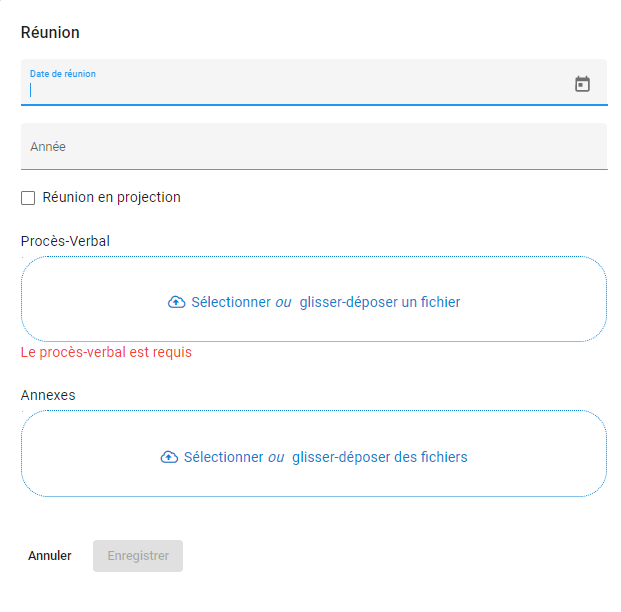
\includegraphics[width=5cm,frame]{Images/catl/cca-pv-new.png}
    \caption{Fenêtre d'encodage d'une nouvelle réunion (PV). }
    \label{fig:cca-pv-new}
\end{figure}



\subsection{Onglet - Composition de la CCA}
Ce volet concerne la composition de votre CCA (voir fig. \ref{fig:cca_compo}). 

\subsubsection{Encoder la composition CCA}
Après avoir défini le \textbf{modèle de composition} (15, 20 ou 25 membres de CCA), il vous est possible de renseigner les différents \textbf{membres effectifs}, \textbf{suppléants} et \textbf{invités} ainsi que leurs coordonnées.  Une zone de téléchargement vous permet également de joindre à la grille de composition les documents annexes nécessaires. 

Pour chaque composante, vous devez cliquer sur \ovalbox{Valider} en bas de la composante concernée pour enregistrer l’encodage effectué. Une fois l’encodage terminé, cliquez sur « Soumettre à l’ONE » pour introduire officiellement la demande de validation de la composition de CCA. 

Le statut de votre composition passe de « \textbf{En cours de composition} » à « \textbf{En cours d’analyse} ». Lorsque l’ONE l’aura validée, le statut de votre composition passera à « \textbf{Validée} ».  

\begin{figure}[htbp]
    \centering
    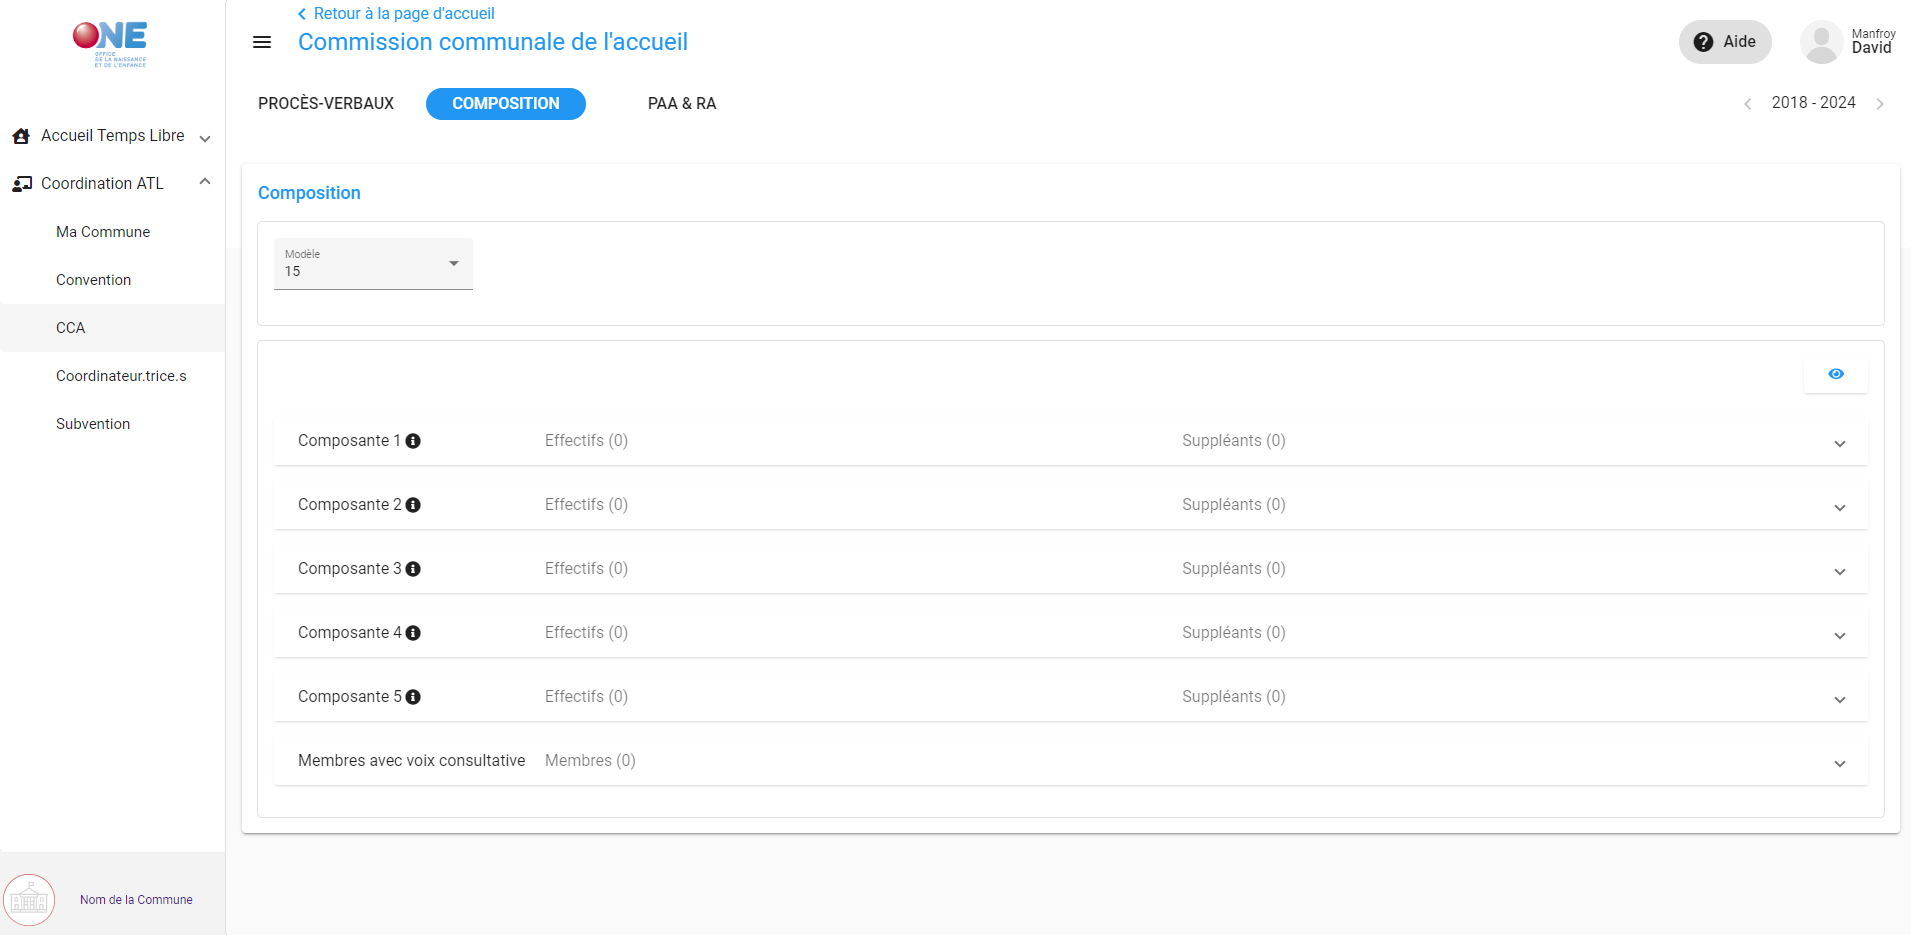
\includegraphics[width=12cm,frame]{Images/catl/cca-compo.png}
    \caption{L'onglet composition de la cca permet d'encoder les personnes qui siègent dans les diverses composantes de la commission.}
    \label{fig:cca_compo}
\end{figure}



%ajout logo
\subsubsection{Télécharger les données encodées}
L’encodage des coordonnées est optionnel, mais vous avez la possibilité ensuite de télécharger la composition de CCA afin de vous en servir comme listing de contacts.


\subsection{Onglet - PAA \& RA}
Dans ce dernier onglet, vous devrez charger les \textbf{plans d’actions annuels} (PAA) et les \textbf{rapports d’activités} (RA). Il faut à chaque fois sélectionner l’année scolaire concernée. 

Comme pour les PV de CCA, nous vous demandons de transmettre les PAA et RA dès que les documents sont réalisés, sans attendre la fin de l’année civile. Pour charger un nouveau document, cliquez sur \ovalbox{+ Nouveau Document}. 

Sélectionnez ensuite l’année scolaire concernée. Précisez s’il s’agit d’un PAA ou d’un RA. N’oubliez pas de cocher la case “Transmis au Conseil communal pour information” si cela a été fait. Déposez enfin votre document dans la zone de chargement et cliquez sur \ovalbox{Ajouter}. 

Un espace commentaire est disponible si vous le souhaitez. Il est visible par les agents ONE. 

\begin{figure}[htbp]
    \centering
    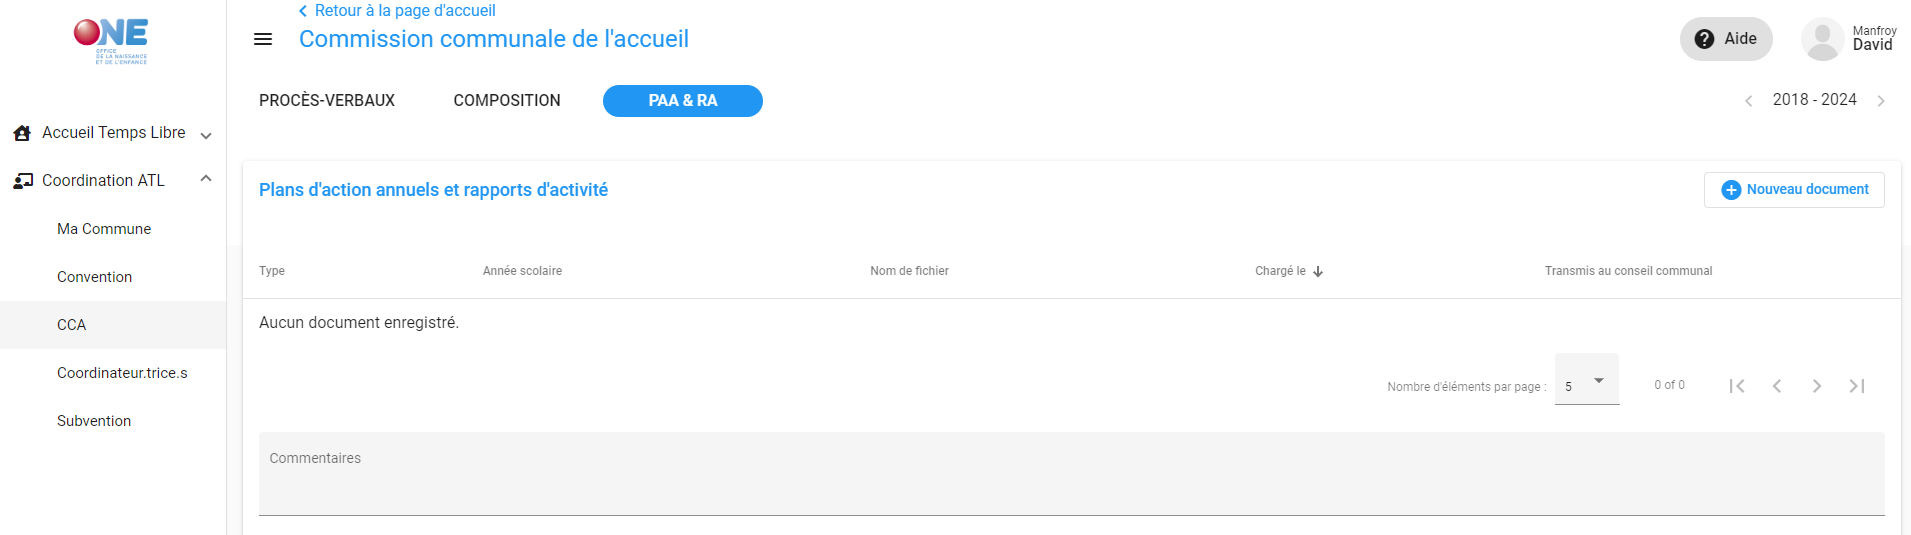
\includegraphics[width=12cm,frame]{Images/catl/cca-paa-ra.png}
    \caption{L'onglet PAA \& RA permet de charger les plan d'actions annuels et les rapports d'activités. Nous vous conseillons à présent de scinder les deux pages du fichier Excel que vous utilisez.}
    \label{fig:cca-paa-ra}
\end{figure}


\begin{information}
Il n’est plus nécessaire de charger la délibération du conseil communal pour les PAA et RA.
\end{information}

\section{Entrée - Coordinateur.trice.s}
L'entrée Coordinateur.trice permet de consulter les Coordinateurs.trices ATL de la Commune. 

Chaque fiche de coordinateur.trice présente plusieurs informations: 
\begin{itemize}
    \item \textbf{les données de contacts et les informations de prestation}: vous renseignerez les informations professionnelles de la coordinatrice ATL. Ces informations sont publiées chaque mois sur le site institutionnel public one.be.
    \item \textbf{Les frais personnels}: il s’agit d’un récapitulatif des \textbf{frais salariaux} (bruts et charges patronales) et \textbf{coûts annexes} liés au poste de coordinateur/trice ATL.
    \begin{itemize}
    \item S’il n’occupe qu’un seul mi-temps ATL dans la commune, les charges salariales seront prises en compte à 100 \%.
    \item S’il occupe un mi-temps ATL et un autre temps de travail au sein de la commune ou ailleurs, les charges salariales ne seront prises en compte qu’à concurrence du mi-temps ATL.
    \item Etc. 
    \end{itemize}
    \item \textbf{Les frais de déplacement}
\end{itemize}


\begin{figure}[htbp]
    \centering
    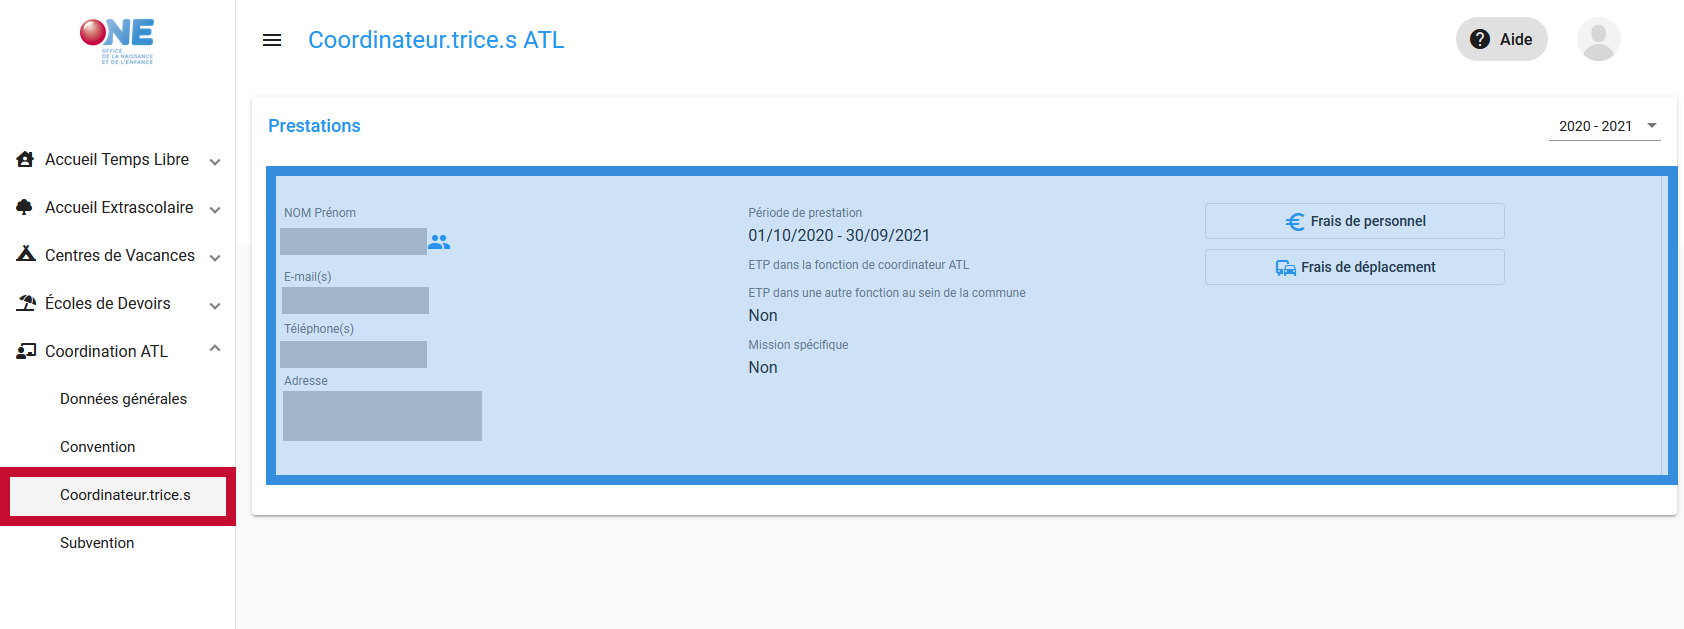
\includegraphics[width=12cm]{Images/catl/catl_prestation.png}
    \caption{Entrée Coordinateur.trice: fiche de vos coordinatrices}
    \label{fig:catl_prestation}
\end{figure}


\subsection{Ajout d'une coordinatrice ATL: création d'une prestation}



\subsubsection{Sélection ou création d'une personne}
En cliquant sur \textbf{Nom Prénom}, une liste déroulante s'affiche avec les personnes renseignées dans "Mon Équipe". 

Si la personne n'est pas présente dans la liste, cliquez sur \ovalbox{Créer une personne}. Au moyen du NISS, ajoutez la personne. Vous devez encoder ensuite le prénom, nom et date de naissance de la personne. La date de naissance sera déduite du NISS. Si besoin, corrigez-la. Vous serez ensuite invité à encoder le contrat de travail de la personne. 

\begin{conseil}
Pour vous aider, suivez le point \ref{team_add_person} "Ajouter une personne dans Mon Équipe".
\end{conseil}

\subsubsection{Sélection ou création du contrat}
    En cliquant sur \textbf{Contrat}, la liste vous donnera l'ensemble des liens contractuels que la personne entretient avec votre pouvoir organisateur. La liste ne vous affichera que les contrats qui sont actifs. 
    \begin{conseil}
     Pour vous aider, suivez le point \ref{team_add_contract} "Ajouter un contrat/un lien".
    \end{conseil}   
    
\vspace{0.5cm}

\begin{tcolorbox}[title=Cas particulier: délégation de la subvention de coordination]
Lorsque le Pouvoir organisateur a délégué la gestion de la subvention à une ASBL de coordination, les étapes d'encodage sont différents. La manipulation 1 doit se réaliser dans le Portail Pro de l'ASBL de coordination; les manipulations 2 et 3 se feront dans celui de la Commune.




\begin{enumerate}
    \item La première étape consiste à \textbf{ajouter la coordinatrice dans l'équipe de l'ASBL de coordination}. En effet, c'est l'ASBL qui est l'employeur officiel de l'ASBL. La coordinatrice est ensuite détachée pour une commune. Suivez le point \ref{team_add_person} et \ref{team_add_contract} de ce guide. Lors de l'ajout du contrat de travail, il sera possible de spécifier la commune de prestation de la personne.
    \item La deuxième étape consiste à \textbf{donner accès au Portail Pro de la Commune} à une ou plusieurs personnes de l'ASBL. Celles-ci pourront alors encoder les données de subventions de coordination ATL. L'administrateur de la Commune doit ajouter les personnes dans les utilisateurs et configurer leur droit (case coordination ATL cochée). De cette manière, la connexion via itsme sera active.
    \item La troisième étape consiste à \textbf{ajouter la prestation de la coordinatrice} dans le Portail Pro.one.be de la Commune. Dans la liste déroulante sera proposée la coordinatrice employée par l'ASBL. Assurez-vous que c'est bien le contrat de travail entre l'ASBL et la personne qui est sélectionnée. Revenez à l'étape 1 si besoin.
\end{enumerate}
\end{tcolorbox}


\section{Données de subventions propres à chaque coordinateur}

\subsection{Frais de personnel}
Pour compléter ces informations, cliquez sur \ovalbox{Frais de personnel} depuis la fiche du coordinateur.
%\subsubsection{Part du salaire selon subvention}


Concernant la \textbf{part du salaire selon subvention (quote-part)},
\begin{itemize}
    \item Si la fiche salariale indique un mi-temps et que la subvention à laquelle vous avez droit est un mi-temps, indiquez 1.
    \item Si la fiche salariale indique un temps plein et que la subvention à laquelle vous avez droit est un mi-temps, indiquez 0,5.
    \item Etc.
\end{itemize}



%\subsubsection{Charges patronales}
Concernant les \textbf{charges patronales}, tenez compte des réductions groupe cible. 

%subsubsection{Cofinancement}
Concernant le \textbf{cofinancement}, indiquez les subventions perçues d’aide à l’emploi (APE, Maribel…).

Divers postes sont également disponibles en bas de la page; complétez-les si besoin. 


Sauvegardez vos données encodées en cliquant sur \ovalbox{Enregistrer} en bas de la page. 


\begin{info}
Vous pouvez copier-coller une ligne à une autre en cliquant sur la petite flèche bleu 
\includegraphics[height=0.4cm]{Images/icon/icon_copy_paste.png} visible en passant la souris dans la case des mois (première colonne).
\end{info}


\begin{figure}[htbp]
    \centering
    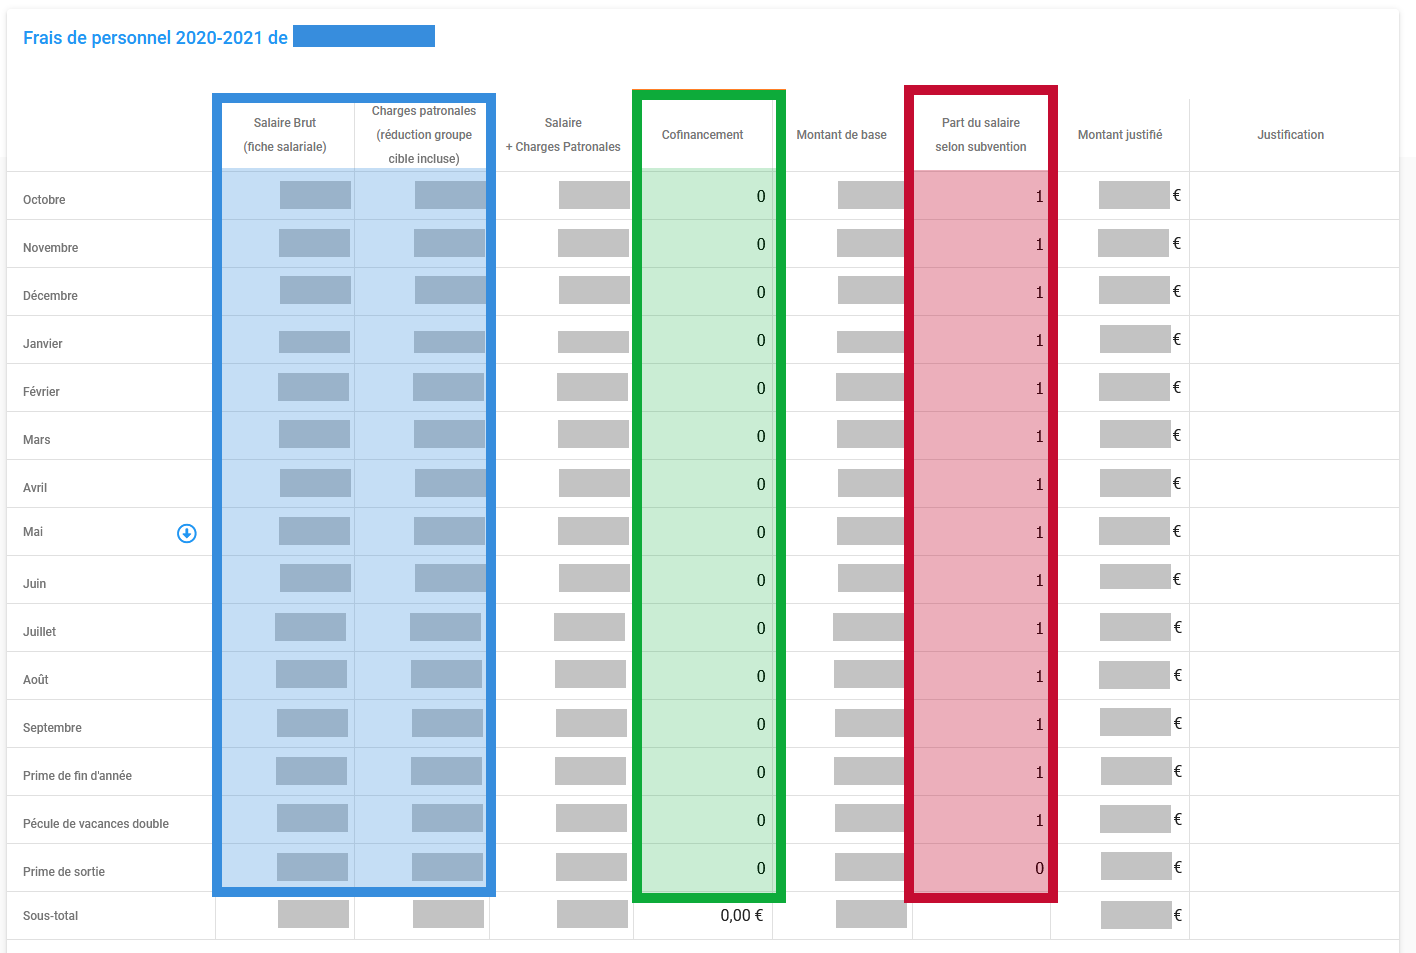
\includegraphics[width=9cm]{Images/catl/frais_personnel.png}
    \caption{Frais de personnel de la coordinatrice ATL}
    \label{fig:catl_frais_personnnel}
\end{figure}



\begin{remarque}
Toutes les charges salariales imputées à la subvention de coordination ATL doivent être liées au temps de travail du CATL.
\end{remarque}

\subsection{Frais de déplacement}
Pour compléter ces informations, cliquez sur \ovalbox{Frais de déplacement} depuis la fiche du coordinateur.

Via le bouton \ovalbox{Frais de déplacement}, encodez un par un vos déplacements. Concernant la distance, il s’agit d’un chiffre entier. Le changement d’index est calculé automatiquement.

\begin{remarque}
L’objet du déplacement doit être suffisamment explicite et uniquement lié aux missions de coordination et/ou aux missions spécifiques.
\end{remarque}


\section{Subvention de coordination ATL}
\subsection{Introduction}
La commune ou l’asbl de coordination doit justifier l’utilisation de la subvention de coordination. 

La subvention de coordination couvre trois types de frais : 
\begin{enumerate}
    \item les frais de personnel du/de la coordinateur/trice ATL, 
    \item ses frais de déplacement,
    \item et les frais de fonctionnement liés à la coordination. 
\end{enumerate}

\subsection{Documents justificatifs à conserver}

L'ensemble des pièces comptables et des documents justificatifs de la subvention doivent rester en vos locaux, à la disposition des inspecteurs comptables pour un contrôle éventuel.


\subsection{Date limite pour introduire votre demande de subsides}
\begin{attention}
La demande de liquidation peut être introduite à partir du 1er octobre, soit après la fin de la période couverte par la subvention\footnote{Période couverte par la subvention: du 1er octobre au 30 septembre de l'année suivante.},  et doit parvenir à l'ONE pour le \textcolor{rouge}{\textbf{31 décembre au plus tard}}.
\end{attention}

%\subsection{Connexion via itsme au Portail Pro.one.be}
%L'administrateur (ou une personne de votre organisation qui possède les droits de gestion des utilisateurs) du Pouvoir organisateur peut ajouter des personnes en tant qu'utilisateur de la plateforme (voir point \ref{gestion_users}). Il faut également configurer les droits "Coordination ATL" (la case Coordination ATL doit être cochée pour le profil concerné). Lorsque le profil est ajouté, la personne aura la possibilité de se connecter au Portail Pro avec l'application itsme ou avec eID.

%begin{conseil}
% Vous pouvez également contacter votre gestionnaire de dossier ONE pour qu'il puisse vous ajouter sur la plateforme https://pro.one.be en tant qu'utilisateur.
%\end{conseil}

\section{Volet Coordination ATL - Entrée Subvention}
Développez le volet Coordination ATL et cliquez sur \ovalbox{Subvention}. Plusieurs onglets sont disponibles: 
\begin{itemize}
    \item \textbf{Frais de fonctionnement}: Il s’agit d’un récapitulatif des frais liés à la fonction de CATL.
    \item \textbf{Résumé}: où vous pourrez envoyer et suivre le statut de votre dossier. 
    \item \textbf{Contact}: la personne de contact que votre gestionnaire de dossier peut contacter en cas de questions.
\end{itemize}

 
\subsection{Le relevé des frais de fonctionnement}
Via l’onglet \ovalbox{Frais de fonctionnement}, encodez vos frais un par un en cliquant sur \ovalbox{Ajouter}.

\begin{figure}[htbp]
    \centering
    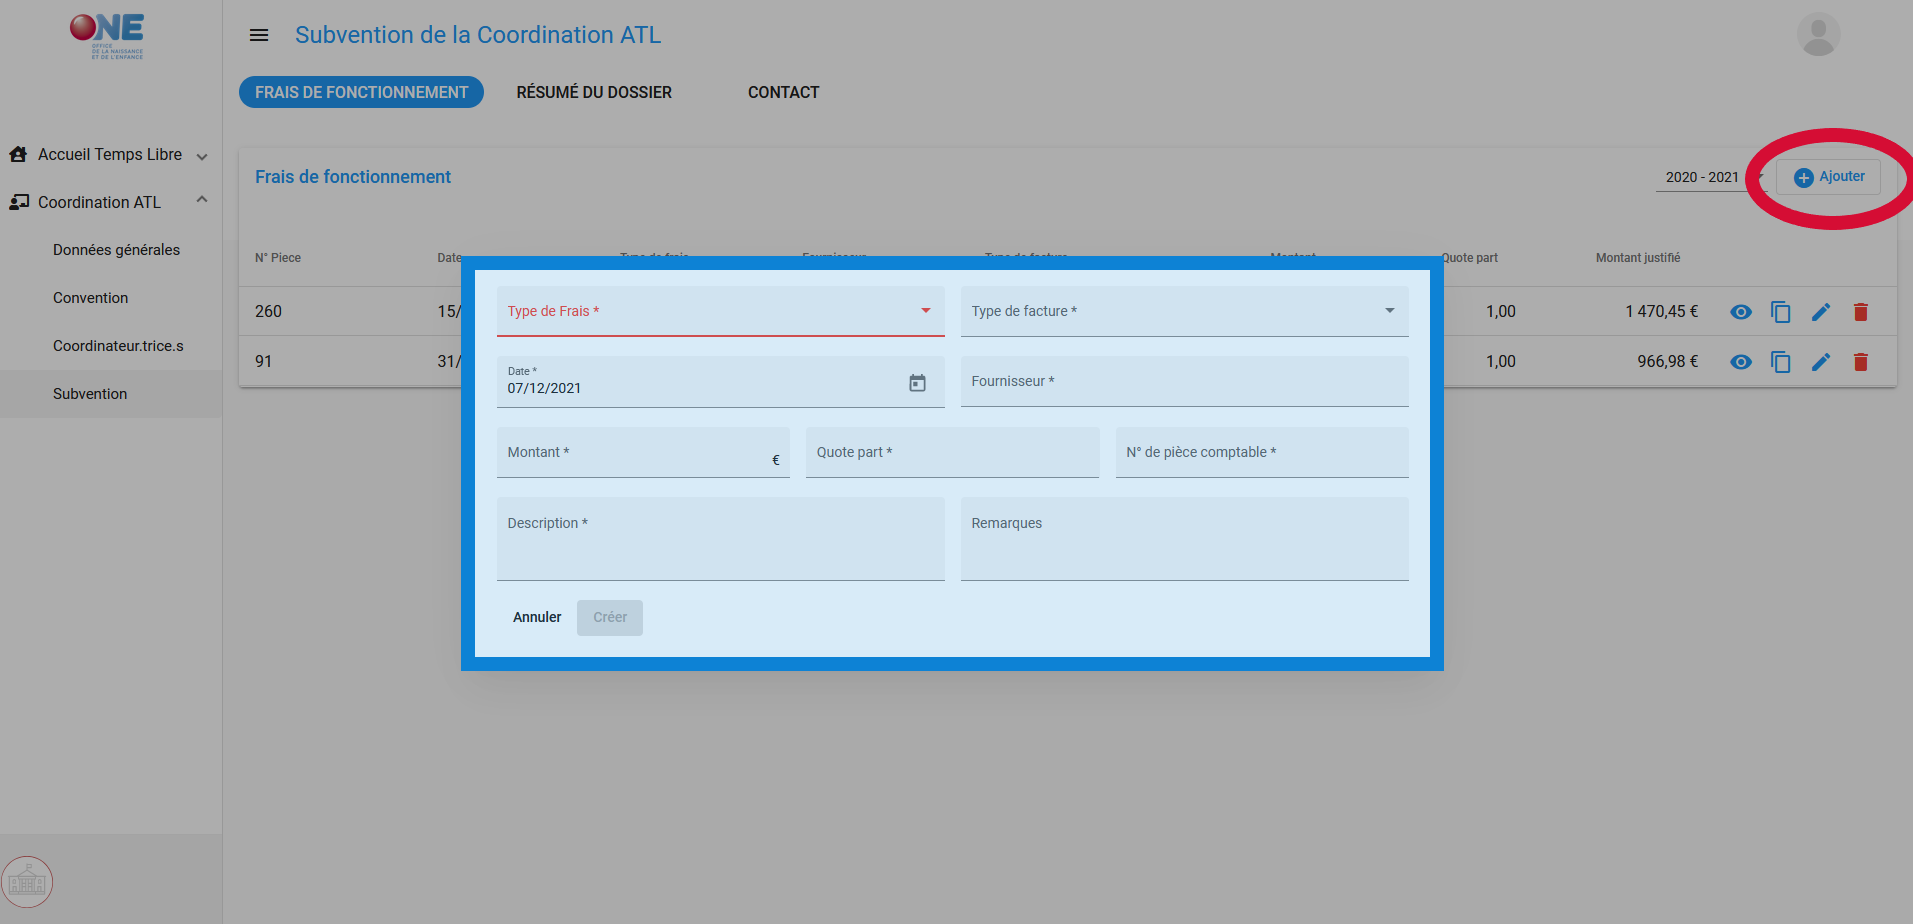
\includegraphics[width=13cm, frame]{Images/catl/frais_fonctionnement.png}
    \caption{Entrée Subvention: ajout d'un frais de fonctionnement}
    \label{fig:catl_frais_fonctionnement}
\end{figure}

\begin{itemize}
    \item Pour certaines factures (eau, gaz, électricité, téléphone, internet, etc...), c'est la date de consommation ou celle de la facture qui est prise en compte.
    \item Pour les factures qui concernent toute la commune ou  l’ASBL, une \textbf{quote-part} sera calculée. Une remarque expliquant la méthode de calcul devra être ajoutée (calcul basé sur un rapport lié au nombre de personnes concernées ou sur un rapport lié à la superficie concernée, ou tout autre calcul cohérent).
        \subitem Exemple : Lorsqu’une facture est 100 \% ATL, la quote-part est 1. Pour une facture globale (commune ou ASBL), avec par exemple, une part CATL de 1/52ème,  la valeur à indiquer = 0,019 (1/52 = 0,019). 
    \item Les réductions ou notes de crédit doivent être prises en compte lors de l’encodage du montant d’une facture à imputer à la subvention (exemple : facture de téléphone ou d’énergie).
\end{itemize}


\begin{info}
Vous pouvez visionner, copier (et éditer), éditer ou supprimer des frais que vous avez ajouté en cliquant sur les icônes de la ligne du frais correspondant.
\end{info}



\subsubsection{Les frais de fonctionnement éligibles}

Les frais de \textbf{courrier}, les frais de \textbf{photocopies}, les frais de \textbf{communication} (téléphone, mailing, internet, fax), les frais de \textbf{fournitures} de bureau,
les frais de \textbf{mobilier de bureau}, les frais de \textbf{matériel informatique} (achat ou leasing), les frais de \textbf{logiciels informatiques}, les frais de \textbf{formation} du (de la) coordinateur(trice) ATL, les frais de \textbf{matériel de présentation} (supports, projecteurs...), les frais d’\textbf{énergie} (eau, gaz, électricité), les frais de \textbf{publication}, les frais de \textbf{réunion}, les frais d’achat de livre ou d’abonnements à des \textbf{publications professionnelles}, les frais de \textbf{jeux et outils didactiques}.



\section{L'envoi du dossier de subvention à l'ONE}
Lorsque votre dossier et vos encodages sont complets, cliquez sur l'entrée \ovalbox{Subvention}, onglet \ovalbox{Résumé}. Le bouton \ovalbox{Introduire ma demande} enverra votre dossier à l'ONE. 


Le bouton ne sera disponible qu'après le remplissage des champs suivants:
\begin{itemize}
    \item données de subvention (frais de personnel et/ou frais de déplacement et/ou frais de fonctionnement);
    \item données de contact des coordinatrices;
    \item données de contact pour le dossier.
\end{itemize}



\begin{information}
Si vous souhaitez modifier votre demande après l'envoi de celle-ci, il sera nécessaire de contacter votre gestionnaire de subvention. L'agent vous renverra votre demande et vous pourrez alors la corriger. N'oubliez pas de renvoyer votre demande une fois les corrections faites.  
\end{information}







